\documentclass{article}

\usepackage{listings}
\usepackage{color}
\usepackage{graphicx}
\usepackage{float}
\usepackage{amsmath}
\usepackage{subfig}
\usepackage{cite}
\usepackage{url}
\usepackage{amsmath}

\newcounter{qcounter}

\begin{document}

\title{Image Analysis - TP5 - Lucas Kanade Tracker}

\author{Jander Nascimento, 
\and Raquel Oliveira}

\maketitle

\section{Initial concept}


\section{Interpolation}

	Bilinear Interpolation is a method to generate a new image (given a initial image {\it I}) where the value of the pixels is a sum of the intensities of its four neighbors, weighted by the distance to the neighbor's center.

	For each pixel {\it(i,j)} of the original image {\it I}, the new pixel in the interpolated image {\it $I_w$} is calculated in the following manner:

	\begin{equation}
		I_w(i+\Delta_i^e , j+\Delta_j^e) += (1-\Delta_i^f)(1-\Delta_j^f)I(i,j)
	\end{equation}
	\begin{equation}
		I_w(i+\Delta_i^e+1 , j+\Delta_j^e) += \Delta_i^f(1-\Delta_j^f)I(i,j)
	\end{equation}
	\begin{equation}
  		I_w(i+\Delta_i^e , j+\Delta_j^e+1) += (1-\Delta_i^f)\Delta_j^fI(i,j)
	\end{equation}
	\begin{equation}
		I_w(i+\Delta_i^e+1 , j+\Delta_j^e+1) += \Delta_i^f \Delta_j^fI(i,j)
	\end{equation}

	where: 
		\begin{itemize}
			\item {\it $\Delta_i$} is the translation along {\it i}
			\item {\it $\Delta_j$} is the translation along {\it j} 
			\item {\it $\Delta^e$} is the integer part of the translation (ie: $\Delta=-5.3$, then ${\it \Delta^e}=-5$
			\item {\it $\Delta^f$} is the decimal part of the translation (ie: $\Delta=-5.3$, then ${\it \Delta^f}=0.3$
		\end{itemize}

	In the Figure \ref{fig:interp} we can see the result of an interpolation. It is possible to observe that the interpolated image, compared with the original image, is a little deformed, due to the fact that the pixels in the new image are interpolated with their neighbors.

	\begin{figure}[H]
		  \centering
		  \subfloat[Original image]{
\includegraphics[width=0.4\textwidth]{img/taz.png}}
		  \hspace{0.1cm}
		  \subfloat[Interpolated image ($\Delta_i=12.8   \Delta_j=-6.3$)]{
\includegraphics[width=0.4\textwidth]{img/taz0interp.png}}
		  \caption{Interpolation of an image}
		  \label{fig:interp}
	\end{figure}	

	After apply a translation ($\Delta_i,\Delta_j$) in an image, we applied the inverse of the translation ($-\Delta_i,-\Delta_j$) on the interpolated image. The result can be seen in the Figure \ref{fig:inverseinterp}. In this figure it is possible to observe that the original image is not achieved when applied the inverse of the interpolation. Although the pixels return to their original position in the image, their intensities are not recovered. Another point to observe is that, when parts of the image are cut by the interpolation (for instance, the foot of Taz), they are not recovered either, due to the fact that they are not in the interpolated image anymore.

	\begin{figure}[H]
		  \centering
		  \subfloat[Original image]{
\includegraphics[width=0.3\textwidth]{img/taz.png}}
		  \hspace{0.1cm}
		  \subfloat[Interpolated image ($\Delta_i=12.8   \Delta_j=-6.3$)]{
\includegraphics[width=0.3\textwidth]{img/taz0interp.png}}
		  \hspace{0.1cm}
		  \subfloat[Inverse of the interpolation]{
\includegraphics[width=0.3\textwidth]{img/taz0interp_inverse.png}}
		  \caption{Inverse of the Interpolation}
		  \label{fig:inverseinterp}
	\end{figure}	


\section{Anaysis of a static image}


\section{Tracking an object}

Here it is a case of Lucas Kanade application.

\begin{figure}[H]
	  \centering
	  \subfloat[Template]{
\includegraphics[width=0.3\textwidth]{../image/report/taz.png}}
	  \caption{Sample Image}
	  \label{fig:template}
\end{figure}	


\begin{figure}[H]
\centering
\subfloat[Template]{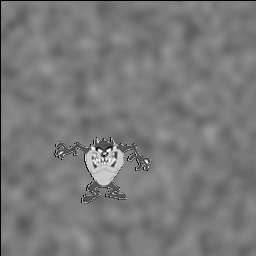
\includegraphics[width=0.3\textwidth]{../image/report/taz004_nb.png}}
		  \hspace{0.1cm}
\subfloat[Template]{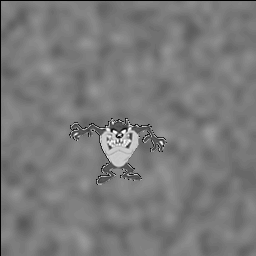
\includegraphics[width=0.3\textwidth]{../image/report/taz020_nb.png}}
		  \hspace{0.1cm}
\subfloat[Template]{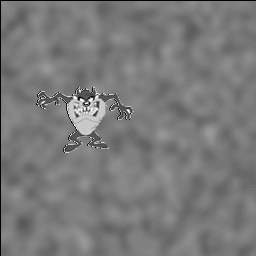
\includegraphics[width=0.3\textwidth]{../image/report/taz063_nb.png}}
\caption{Original Image}
\label{fig:original}
\end{figure}	


\begin{figure}[H]
\centering
\subfloat[Template]{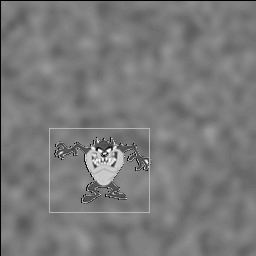
\includegraphics[width=0.3\textwidth]{../image/report/taz004_bb.png}}
		  \hspace{0.1cm}
\subfloat[Template]{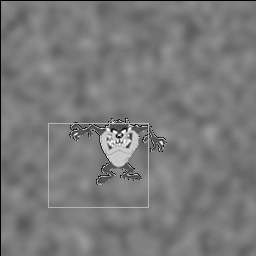
\includegraphics[width=0.3\textwidth]{../image/report/taz020_bb.png}}
		  \hspace{0.1cm}
\subfloat[Template]{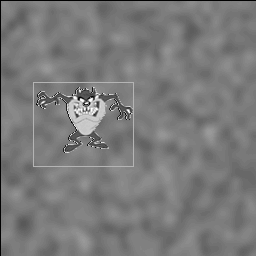
\includegraphics[width=0.3\textwidth]{../image/report/taz063_bb.png}}
\caption{Tracked Images}
\label{fig:original}
\end{figure}	


\section{Drawbacks}

Lucas Kanade has shown to be very efficient in some cases, now let's take a look in the situation where this algorithm does not work that well.

In large motions (at a higher speed) the tracker is not able to detect the changing region of the image with the correct direction vector.

If the image changes drastically its illumination, this can produce a wrong image evaluation.


\section{How to run?}

	Steps to compile the application:
	
	\begin{itemize}
		\item svn checkout https://jfimageanalysis.googlecode.com/svn/trunk/TP5/ \#download source code
		\item make \#compiles the code
	\end{itemize}

	As an input image only a set of {\bf ppm plaintext/ansii} files (P3). 

	Examples of usage:

	\begin{itemize}
		\item ./tp5
	\end{itemize}

	Thre resulting images will be generated in \emph{SRC/image/tazplain}.

\end{document}


